\chapter{Bevezetés} % User guide
\label{ch:bevezetes}

\section{A szükséges programok telepítése}

Code::blocks fejlesztői környezetre és c++ compiler-re (fordító program) lesz szükségünk, amelyeket egy csomagban le is tölthetünk és telepíthetünk a code::blocks oldaláról: \url{https://sourceforge.net/projects/codeblocks/}. Jelenleg erről a linkről windows-ra tölthetjük le a code::blocks-ot c++ fordító programmal együtt. 

Amennyiben valami miatt ez a link nem működne, \url{https://www.codeblocks.org/downloads/} linken válasszuk ki a "Download the binary release" menüpontot.

% TODO: \usepackage{graphicx} required
\begin{figure}[H]
	\centering
	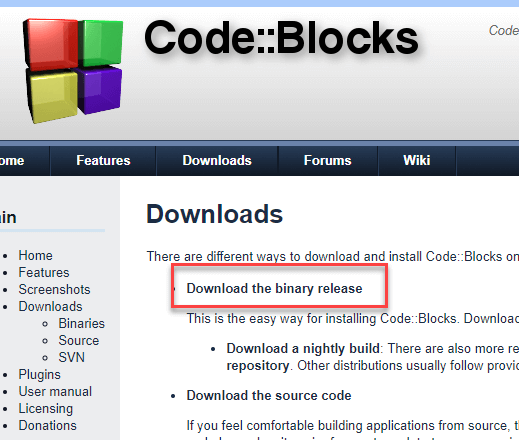
\includegraphics[width=0.6\linewidth]{images/bevezetes/choose}
	\caption{"Download the binary release"}
	\label{fig:choose}
\end{figure}
